%%%%%%%%%%%%%%%%%%%%%%%%%%%%%%%%%%%%%%%%%
% Journal Article
% LaTeX Template
% Version 1.4 (15/5/16)
%
% This template has been downloaded from:
% http://www.LaTeXTemplates.com
%
% Original author:
% Frits Wenneker (http://www.howtotex.com) with extensive modifications by
% Vel (vel@LaTeXTemplates.com)
%
% License:
% CC BY-NC-SA 3.0 (http://creativecommons.org/licenses/by-nc-sa/3.0/)
%
%%%%%%%%%%%%%%%%%%%%%%%%%%%%%%%%%%%%%%%%%

%----------------------------------------------------------------------------------------
%	PACKAGES AND OTHER DOCUMENT CONFIGURATIONS
%----------------------------------------------------------------------------------------

\documentclass[10pt]{article} % Single column

%\documentclass[twoside,twocolumn]{article} % Two column

\usepackage{blindtext} % Package to generate dummy text throughout this template 

\usepackage[sc]{mathpazo} % Use the Palatino font
\usepackage[T1]{fontenc} % Use 8-bit encoding that has 256 glyphs
\linespread{1.05} % Line spacing - Palatino needs more space between lines
\usepackage{microtype} % Slightly tweak font spacing for aesthetics

\usepackage[spanish]{babel} % Language hyphenation and typographical rules

\usepackage[hmarginratio=1:1,top=32mm,columnsep=20pt]{geometry} % Document margins
\usepackage[hang, small,labelfont=bf,up,textfont=it,up]{caption} % Custom captions under/above floats in tables or figures
\usepackage{booktabs} % Horizontal rules in tables

\usepackage{lettrine} % The lettrine is the first enlarged letter at the beginning of the text

\usepackage{enumitem} % Customized lists
\setlist[itemize]{noitemsep} % Make itemize lists more compact

\usepackage{abstract} % Allows abstract customization
\renewcommand{\abstractnamefont}{\normalfont\bfseries} % Set the "Abstract" text to bold
\renewcommand{\abstracttextfont}{\normalfont\small\itshape} % Set the abstract itself to small italic text

\usepackage{titlesec} % Allows customization of titles
\renewcommand\thesection{\Roman{section}} % Roman numerals for the sections
\renewcommand\thesubsection{\roman{subsection}} % roman numerals for subsections
\titleformat{\section}[block]{\large\scshape\centering}{\thesection.}{1em}{} % Change the look of the section titles
\titleformat{\subsection}[block]{\large}{\thesubsection.}{1em}{} % Change the look of the section titles

\usepackage{fancyhdr} % Headers and footers
\pagestyle{fancy} % All pages have headers and footers
\fancyhead{} % Blank out the default header
\fancyfoot{} % Blank out the default footer
\fancyhead[C]{Compilaci\'on. \textbf{Cool Compiler 2023}} % Custom header text
\fancyfoot[RO,LE]{\thepage} % Custom footer text

\usepackage{titling} % Customizing the title section

\usepackage{hyperref} % For hyperlinks in the PDF

\usepackage{graphicx} % For images

\usepackage{pifont} % bullets

\usepackage{amsmath}

\usepackage{algpseudocode}

\usepackage{float}
% Keywords command
\providecommand{\keywords}[1]
{
	\small	
	\vspace{0.5em}
	\noindent \textbf{\textit{Palabras clave --- }} #1
}


%----------------------------------------------------------------------------------------
%	TITLE SECTION
%----------------------------------------------------------------------------------------

\setlength{\droptitle}{-4\baselineskip} % Move the title up

\pretitle{\begin{center}\Huge\bfseries} % Article title formatting
	\posttitle{\end{center}} % Article title closing formatting
\title{\normalsize{Compilaci\'on}\\
	\Huge\bfseries Cool Compiler 2023 \\
} % Article title
\author{% 
	
\includegraphics[width=15em]{logo.png}\\
	Karlos Alejandro Alfonso Rodríguez\\
	Laura Victoria Riera P\'erez\\
	Kevin Talavera Díaz \vspace{1em} \\
	\small Cuarto a\~no. Ciencias de la Computaci\'on. \\ % institution
	\small Facultad de Matem\'atica y Computaci\'on, Universidad de La Habana, Cuba \\ % institution
}
\date{\footnotesize \today } % Leave empty to omit a date


% Abstract configurations
\renewenvironment{abstract}
{\small
	\begin{center}
		\bfseries \abstractname\vspace{-.5em}\vspace{0pt}
	\end{center}
	\list{}{
		\setlength{\leftmargin}{1.5cm}%
		\setlength{\rightmargin}{\leftmargin}%
	}%
	\item\relax}
{\endlist}

\usepackage{amsthm}
\usepackage{amssymb}
\usepackage{todonotes} % \TODO
\usepackage{listings} % Code listings
\usepackage{xcolor}

\definecolor{backcolour}{rgb}{0.95,0.95,0.92}

\newcommand{\csl}[1]{\colorbox{backcolour}{\texttt{#1}}}

\newcommand{\imgcaption}[2]{\tiny \textbf{Figura #1.} #2.}

\newcommand{\mgc}[2][]{\colorbox{backcolour}{\texttt{\_\_#2\_\_#1}}}

\newcommand{\mgccapt}[1]{\texttt{\_\_#1\_\_}}

\newtheorem{thm}{Teorema}
\newtheorem{mydef}{Definici\'on}%[section]
\newtheorem{lem}{Lema}
\newtheorem{fig}{\scriptsize{Figura}}


\renewcommand{\qedsymbol}{\rule{0.7em}{0.7em}}

% Hyperlinks configurations
\hypersetup{
	colorlinks=true,
	linkcolor=black,
	filecolor=magenta,      
	urlcolor=cyan,
	pdftitle={Overleaf Example},
	pdfpagemode=FullScreen,
}

%----------------------------------------------------------------------------------------

\begin{document}
	
	\bibliographystyle{ieeetr}
	
	% Print the title
	\maketitle
	
	%----------------------------------------------------------------------------------------
	%	ARTICLE CONTENTS
	%----------------------------------------------------------------------------------------
	
	\section*{Repositorio del proyecto}
	\begin{center}
		\url{https://github.com/computer-science-crows/cool-compiler-2023}
	\end{center}

	\section{Uso del compilador}
	
	Para utilizar el compilador, navegue al directorio /src y ejecute el siguiente comando: \textit{python -m coolcmp -h}, lo que mostrará la ayuda con las opciones disponibles. Para compilar el archivo \textit{code.cl}, simplemente ejecute: \textit{python -m coolcmp code.cl}. Este proceso generará un archivo \textit{code.mips}, que puede ser ejecutado en el simulador SPIM mediante el comando: \textit{spim -f code.mips}.
	
	\begin{figure}
		\centering
		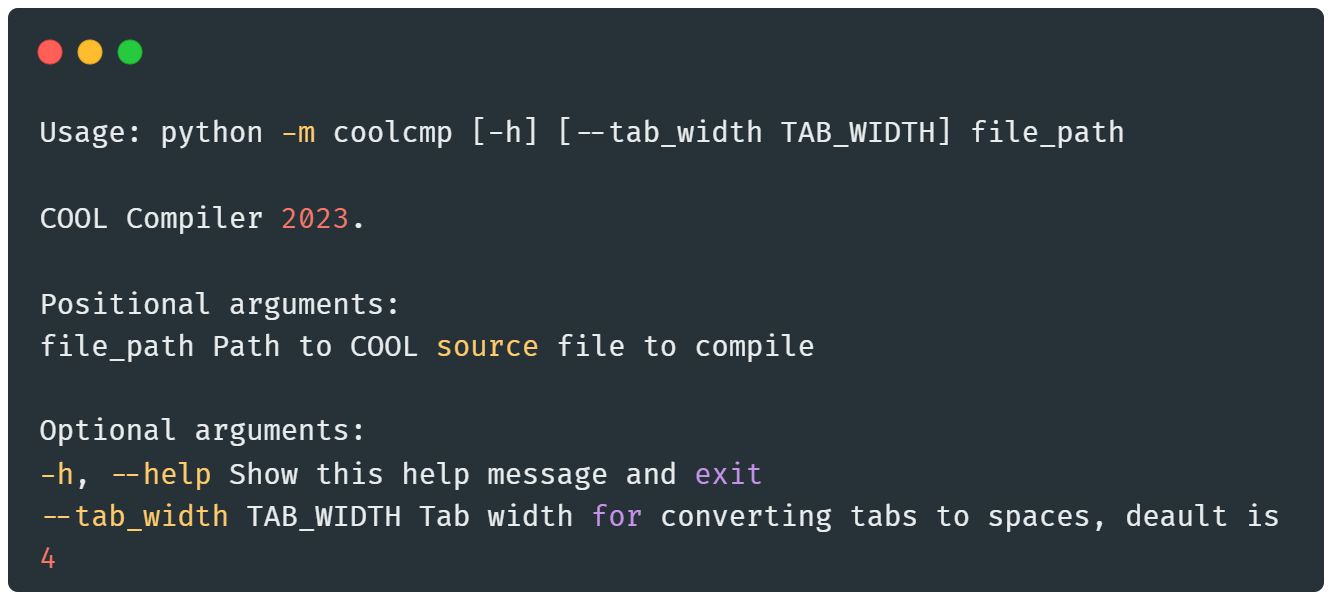
\includegraphics[width=10cm]{usage}
		\caption{Uso del compilador}
	\end{figure}

	\subsection{M\'odulos}
	
	El proyecto está estructurado en varios módulos ubicados en la carpeta /src:
	
	\begin{figure}[H]
		\centering
		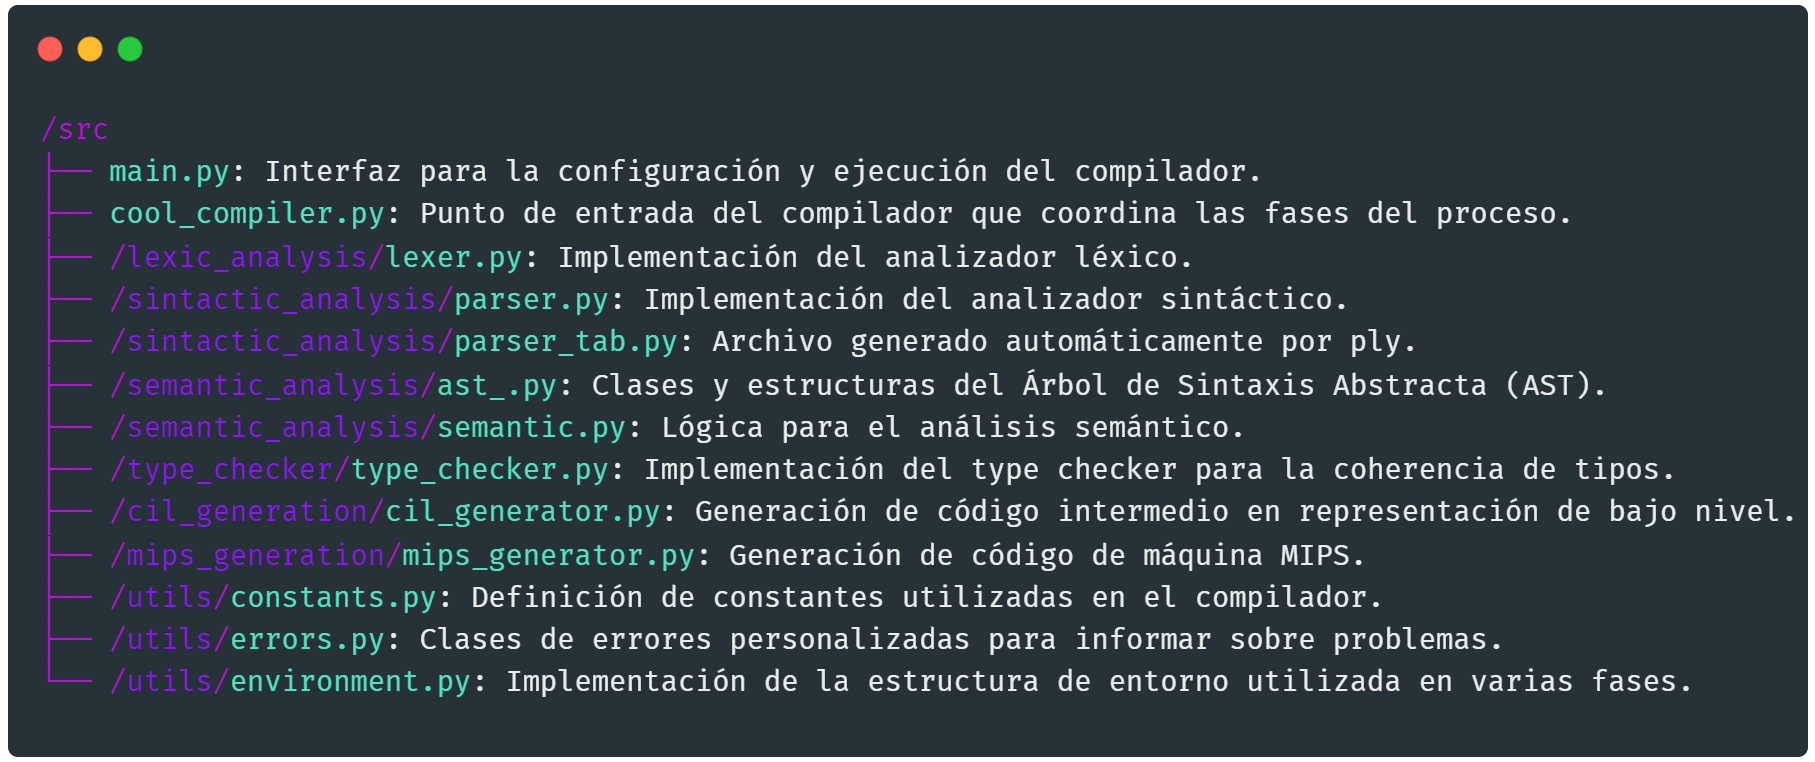
\includegraphics[width=15cm]{structure}
		\caption{Estructura del proyecto}
	\end{figure}

	\subsection{Fases}
	
	El proceso de compilación consta de varias fases esenciales que transforman el código fuente en COOL en un programa ejecutable. Comienza con el análisis léxico, donde se identifican los componentes básicos del código. Luego, el análisis sintáctico verifica la estructura gramatical correcta. A continuación, el análisis semántico evalúa el significado del código. El chequeo de tipos garantiza la coherencia entre los tipos en el programa. La generación de código intermedio crea una representación más abstracta del programa. Finalmente, la generación de código de máquinas traduce el programa a instrucciones específicas del hardware para su ejecución. 
	
	\begin{figure}[H]
		\centering
		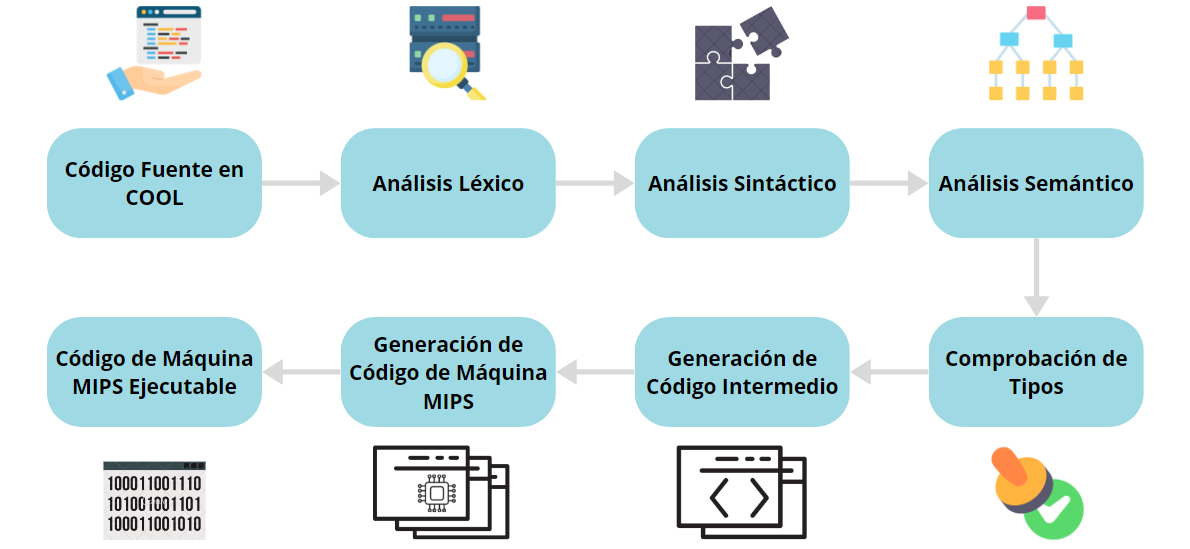
\includegraphics[width=13.5cm]{flow}
		\caption{Flujo del programa}
	\end{figure}
	
	\subsubsection{An\'alisis L\'exico}
	
	En el proceso de análisis léxico, se ha aprovechado la versatilidad de la biblioteca PLY (Python Lex-Yacc) para simplificar la definición de tokens y reglas en la implementación del lexer. La primera tarea implica la categorización de tokens, abarcando identificadores, palabras clave, literales y operadores, que son las unidades léxicas fundamentales en el lenguaje COOL. Estas categorías se definen mediante expresiones regulares, estableciendo reglas específicas para cada tipo de token. Es destacable la atención especial dedicada a las reglas diseñadas para manejar comentarios y cadenas de caracteres.
	
	En la lógica de creación de tokens, se emplea la funcionalidad de la pila de estados de PLY, permitiendo la transición fluida entre contextos al detectar el inicio de comentarios o cadenas de caracteres. Este enfoque adaptativo posibilita la aplicación de reglas específicas según la situación y la restauración al estado anterior al completar cada sección particular. Además, el código del lexer está equipado con un sólido mecanismo de manejo de errores. Detecta y registra posibles problemas léxicos, como comentarios no cerrados o cadenas de caracteres no terminadas, proporcionando una capa adicional de robustez al proceso de análisis.
	
	\subsubsection{An\'alisis Sint\'actico}
	
	La fase de análisis sintáctico se ha llevado a cabo mediante el uso de la herramienta PLY (Python Lex-Yacc). Inicialmente, se convirtió la gramática de COOL de su forma extendida en la notación de Backus-Naur a la forma estándar. Posteriormente, se generó un esqueleto del archivo `parser.py` que contiene cada regla gramatical como un método dentro de la clase `Parser`. Este enfoque es necesario para la correcta integración con PLY.
	
	Cada método del parser se completa con la parte derecha de la regla correspondiente. Se crearon clases para modelar cada símbolo de la gramática, representando así los nodos del Árbol de Sintaxis Abstracta (AST). Estas clases se han diseñado para incluir información sobre la línea y columna en la que se encuentra el símbolo correspondiente en el código fuente.
	
	Las reglas del parser abordan distintos aspectos de la gramática de COOL, desde la definición de programas y clases hasta la manipulación de expresiones y operaciones. Por ejemplo, se definen reglas para la construcción de clases, métodos, atributos, expresiones condicionales, bucles, y más.
	
	Además, se han establecido prioridades y asociatividades entre operadores para resolver posibles conflictos durante el análisis sintáctico. Se ha incorporado también manejo de errores en caso de que la gramática no sea seguida adecuadamente, generando excepciones que informan sobre la presencia y ubicación de posibles errores sintácticos.
	
	\subsubsection{An\'alisis Sem\'antico}
	
	En el contexto del análisis semántico en el compilador de COOL, se inicia verificando las reglas semánticas especificadas en el manual del lenguaje. Un componente esencial de esta fase es la construcción del árbol de herencia, donde cada nodo representa una clase y las relaciones de herencia se establecen a través de nodos hijos. Este árbol se inicia desde la clase base "Object", y se implementa un algoritmo de búsqueda en profundidad (DFS) para detectar posibles ciclos, asegurando así que el árbol sea acíclico, como exige COOL.
	
	Una tarea crítica es la gestión de SELF\_TYPE. Se establecen las siguientes relaciones de conformance: SELF\_TYPEX $\leq$ SELF\_TYPEX (reflexividad) y SELF\_TYPEC $\leq$ P si C $\leq$ P (transitividad). Para manejar SELF\_TYPE, se agrega un nodo SELF\_TYPEC como hijo de cada nodo C en el árbol de herencia, garantizando la conformidad para casos reflexivos y transitivos.
	
	La construcción del árbol de herencia también implica la detección de posibles errores, como la redefinición de clases y la validación de herencias desde clases no definidas. Se garantiza que las clases estén ordenadas en el árbol según sus líneas en el código fuente, contribuyendo a un análisis semántico coherente.
	
	Además, se verifica la consistencia de métodos y atributos en las clases. Se implementa un proceso de comprobación para evitar la redefinición no permitida de métodos y atributos. También se realiza una verificación específica para asegurar la existencia de la clase "Main" y la presencia del método "main" en esta clase, sin recibir argumentos.
	
	\subsubsection{Comprobaci\'on de Tipos}
	
	El chequeo de tipos se realiza utilizando el patrón de diseño Visitor para proporcionar una estructura modular y extensible. Este patrón permite separar las operaciones específicas de los nodos del Árbol de Sintaxis Abstracta (AST) en clases independientes conocidas como visitantes. Esta separación de responsabilidades facilita la extensión del compilador sin modificar directamente las clases de los nodos del AST, proporcionando una organización clara y simplificando el mantenimiento del código.
	
	En el contexto del Chequeo de Tipos, cada clase de nodo en el AST implementa un método accept que acepta un visitante como argumento. Cada visitante tiene métodos específicos para realizar operaciones particulares en los nodos del AST. Por ejemplo, para el Conformance Test, se utiliza un visitante que realiza un recorrido DFS asignando tiempos de descubrimiento y finalización, permitiendo una verificación eficiente de la conformidad de tipos. Además, otro visitante se encarga de responder preguntas sobre el Lowest Common Ancestor, esencial para operaciones como "join". Este enfoque modular y basado en el patrón Visitor contribuye a la flexibilidad y mantenibilidad del compilador COOL.
	
 	Previo al análisis de tipos, es esencial realizar la \textbf{verificación de conformidad de tipos}. En este contexto, se dice que un nodo U \textit{conforma} con otro nodo V si el nodo U puede ser manejado como si perteneciera al tipo del nodo V. Durante esta validación, se asegura que las expresiones y operaciones del programa sigan las reglas de tipos establecidas por COOL, posibilitando el polimorfismo al permitir que objetos de clases derivadas se utilicen en contextos donde se espera una clase base. La conformidad de tipos se establece en función del árbol de herencia, donde un tipo se considera conforme a otro si comparten el mismo tipo o están en su cadena de herencia. 
	
	Para llevar a cabo esta tarea, se emplea un Depth-First Search (DFS) que calcula dos valores para cada nodo $x$: $td(x)$, el tiempo de descubrimiento de $x$, es decir, el primer momento en que el DFS llega a X; y $tf(x)$, el tiempo de finalización de $x$, es decir, el último momento en que el DFS está en $x$. La relación de conformidad entre dos nodos $U$ y $V$ se verifica mediante las propiedades de $td$ y $tf$. $U$ conforma con $V$ si $td(V) \leq td(U) \leq tf(V)$.
	
	La operación \textit{join} en COOL se utiliza para determinar el tipo estático común más bajo de dos tipos dados. Esta operación es necesaria cuando se realiza una operación de "dispatch" o llamada a método en COOL para garantizar que se esté invocando el método correcto según la jerarquía de tipos. Para encontrar el tipo estático común más bajo, se utiliza el concepto de \textbf{Lowest Common Ancestor} (LCA) o ancestro común más bajo de dos nodos en el AST. La implementación sigue un proceso básico: si el nodo U está más lejos de la raíz que el nodo V, se establece que LCA(U, V) = LCA(padre(U), V). Este proceso se repite hasta que U y V son iguales, momento en el cual el LCA es U. 
	
%	 \textbf{Inicialización del Orden:}
%	Durante la traversa DFS del AST, se inicializan los valores td y tf para cada nodo. Además, se verifican las compatibilidades de los métodos heredados y se precálcula el tipo estático de los formales de los métodos antes de la visita.
%
%	 \textbf{Resolución de Problemas Técnicos:}
%	
%	Conformidad de Métodos Inherentes: Se asegura que los métodos heredados sean compatibles con los métodos en la clase hija.
%	
%	Ciclos en la Herencia: Se verifica la presencia de ciclos durante la construcción del árbol de herencia.
%	
%	Consideraciones
%	Ambiente de Tipos: Se mantiene un entorno actual (current\_environment) durante el recorrido del AST para realizar comprobaciones de tipos.
%	
%	Ámbito de Clases: Se realiza un seguimiento del ambiente de clases actual (current\_class) para lidiar con herencias y definiciones de clases.
	
	\subsubsection{Generaci\'on de C\'odigo Intermedio}
	
	La \textbf{representación de clases} en el proceso de generación de código MIPS implica la transformación de cada clase en una función de inicialización, denominada ``FuncInit''. Esta función tiene la responsabilidad de crear instancias de la clase correspondiente cuando se llama en código MIPS. Las clases contienen una serie de \textbf{atributos}, entre ellos los atributos reservados como "\_type\_info", que almacena la referencia a la dirección de memoria que contiene los datos del tipo de la instancia, y "\_size\_info", que indica la cantidad de bytes que la instancia ocupará en memoria. Existen atributos específicos para clases particulares, como "\_int\_literal" para la clase "Int", que representa el entero asociado a la instancia, y "\_string\_length", "\_string\_literal" para la clase "String", que almacenan la longitud y el contenido de la cadena, respectivamente. Por último, "\_bool\_literal" en la clase "Bool" contiene un valor booleano (1 para "true" o 0 para "false"). Además de los atributos reservados, las clases pueden tener atributos adicionales declarados por el programador durante la definición de la clase.
	
	Un aspecto clave es el almacenamiento de tiempos de descubrimiento (td(C)) y finalización (tf(C)) para cada clase. Estos tiempos son cruciales para la resolución de dispatches, es decir, llamadas a métodos, ya que determinan la ubicación de la implementación del método en la jerarquía de clases. También son fundamentales en expresiones Case, donde los tiempos de descubrimiento y finalización facilitan la resolución de las diversas ramas del caso. 
	
	La \textbf{representación de métodos} en el proceso de generación de código MIPS implica la transformación de cada método, denotado como "f", en una "función" (Function). Cuando un método "f" está definido en una clase "C", se registran datos esenciales asociados a esa función, incluyendo los tiempos de descubrimiento (td(C)), finalización (tf(C)), y el nivel (level) de la clase "C" en el árbol de herencia. Estos datos son cruciales para la gestión de dispatches y otras resoluciones durante la ejecución del programa.
	
	La función resultante encapsula la lógica y comportamiento del método, y su identificador está compuesto por el nombre de la clase que la contiene seguido por el nombre del método, proporcionando así una forma única de referenciar la función. La información sobre tiempos y niveles se utiliza especialmente en dispatches, donde se requiere una resolución dinámica y eficiente de la llamada a métodos. El nivel indica la distancia desde la raíz del árbol de herencia, lo que facilita la determinación de la clase correcta a la que pertenece el método, mientras que los tiempos de descubrimiento y finalización son fundamentales para garantizar el orden adecuado de ejecución y la coherencia en la resolución de expresiones.
	
	La \textbf{asignación de posiciones a variables en el stack} es un paso crítico en el proceso de generación de código MIPS. Cada variable, ya sea una variable de clase (atributo) o una variable local (parámetro formal, variable Let o Case), debe tener una posición predefinida en el stack para garantizar su acceso eficiente durante la ejecución del programa.
	
	Este proceso se lleva a cabo mediante la creación y gestión de un entorno, que es una estructura que mantiene un mapeo entre el nombre de cada variable y su posición correspondiente en el stack. El entorno también tiene un padre, que representa el bloque en el que se encuentra actualmente. Al llegar a bloques como Let, CaseBranch, FuncInit o Function, se crea un nuevo entorno. En la definición de una variable, ya sea en el entorno actual o en bloques superiores, se asigna la posición adecuada y se incrementa el contador de posiciones.
	
	Durante el proceso, se registran las referencias a las variables, indicando si se refieren a atributos de clase o a variables locales. Cuando se sale de un bloque, el entorno se reinicia al padre correspondiente, y se ajustan las posiciones según el estado previo. Este enfoque garantiza una gestión coherente y eficiente de las variables en el stack, facilitando su acceso y manipulación durante la ejecución del programa.
	
	\subsubsection{Generaci\'on de C\'odigo de M\'aquina}

	En la etapa final de la compilación de COOL, la generación de código MIPS se lleva a cabo con una implementación meticulosa de las funcionalidades detalladas en el manual.
	
	Para la gestión de registros, se adoptó una estrategia sencilla pero efectiva. Un registro se dedica exclusivamente a contener la dirección de memoria del objeto self actual. Los registros temporales se emplean para operaciones temporales, y se reservan registros específicos para "pasar" y "regresar" referencias de objetos. Cuando es necesario manipular más de un argumento o valor, se recurre al uso de la pila (stack) de MIPS.
	
	La resolución de dispatches, que implica la llamada a métodos en tiempo de ejecución, se lleva a cabo eficientemente. Se almacena información esencial sobre las funciones con nombre f en el Data Segment, organizadas por nivel en orden descendente. Resolver un dispatch implica buscar el ancestro más profundo de la clase actual (C) que contenga una función con nombre f. La complejidad de esta operación es O(\#funciones distintas).
	
	El proceso de resolución de expresiones Case sigue un enfoque similar al de los dispatches. Las ramas se reorganizan según el ancestro más profundo, y la resolución se reduce a buscar el primer ancestro que sea un caso válido para la expresión.
	
	En relación con los Strings y el Data Segment, se almacenan literales de Int, String y Bool en este segmento. Para cumplir con el alineamiento requerido por MIPS, se añaden ceros a los literales de String, asegurando que su tamaño sea un múltiplo de 4.
	
\end{document}


